\PassOptionsToPackage{dvipsnames}{xcolor}
\documentclass[final]{beamer}

\usepackage[T1]{fontenc}
\usepackage{lmodern}

% set poster dimensions below (in cm)
% AFI / the posterboards at the Discovery Building are 46"x46".
% 46" wide x 36" high (121.92 x 91.44 cm)
% A0 for ASA WI Chapter, which is slightly smaller 84.1 x 118.9
\usepackage[size=custom,width=118.9,height=84.1, scale=1]{beamerposter}
\usetheme{gemini}
\usecolortheme{mit}
\usepackage{graphicx}
\usepackage{tikz}
\usepackage{xcolor}

\usepackage[backend=bibtex, sortcites, style=authoryear]{biblatex}
\addbibresource{references.bib}

% https://tex.stackexchange.com/questions/585635/beamer-biblatex-authoryear-causes-problem-with-insertbiblabel
\setbeamertemplate{bibliography item}{}


\usepackage{tikz}
\usepackage[protrusion=true,expansion=true]{microtype}
\usepackage{anyfontsize}
\usepackage{hyperref}

\usepackage{hayesmacros}
\usepackage{amsmath}
\usepackage{amsthm}

\newtheorem{proposition}{Proposition}

% ====================
% Lengths
% ====================

% If you have N columns, choose \sepwidth and \colwidth such that
% (N+1)*\sepwidth + N*\colwidth = \paperwidth
\newlength{\sepwidth}
\newlength{\colwidth}
\setlength{\sepwidth}{0.025\paperwidth}
\setlength{\colwidth}{0.3\paperwidth}

\newcommand{\separatorcolumn}{\begin{column}{\sepwidth}\end{column}}

% ====================
% Title
% ====================

\title{Linear-in-means models may be inestimable even when identified}

\author{Alex Hayes \inst{1} \and Keith Levin \inst{1}}

\institute[shortinst]{\inst{1} Department of Statistics, University of Wisconsin-Madison}

% ====================
% Footer (optional)
% ====================

% \footercontent{\hfill \href{https://www.alexpghayes.com}{https://www.alexpghayes.com}}
% (can be left out to remove footer)

% ====================
% Logo (optional)
% ====================

% use this to include logos on the left and/or right side of the header:
\logoright{
\includegraphics[height=7cm]{figures/logos/color-flush-UWlogo-print.pdf}}

% ====================
% Body
% ====================

\begin{document}

\begin{frame}[t]
    \begin{columns}[t]
        \separatorcolumn

        \begin{column}{\colwidth}

            \begin{alertblock}{Abstract}

                Linear-in-means models are widely used to investigate peer effects. Identifying peer effects in these models is challenging, but conditions for identification are well-known. However, even when peer effects are identified, they may not be estimable, due to an asymptotic colinearity issue: as sample size increases, peer effects become more and more linearly dependent.  We show that asymptotic colinearity occurs whenever nodal covariates are independent of the network and the minimum degree of the network is growing. Asymptotic colinearity can cause estimators to be inconsistent or to converge at slower than expected rates. We also demonstrate that dependence between nodal covariates and network structure can alleviate colinearity issues in random dot product graphs. These results suggest that linear-in-means models are less reliable for studying peer influence than previously believed.

            \end{alertblock}

            \begin{block}{The linear-in-means model}


                The linear-in-means model is a canonical approach to estimating social influence in social networks. Suppose there is a network with $n$ nodes, encoded by a symmetric adjacency matrix $A \in \R^{n \times n}$. In binary networks, $A_{ij} = 1$ if nodes $i$ and $j$ form an edge, and $A_{ij} = 0$ otherwise, though we note that our results do not require that $A$ be binary. Each node $i$ is associated with an outcome $Y_i \in \R$ and a covariate $T_i \in \R$. Letting $\Ni = \left\{ j \in [n]: A_{ij} = 1 \right\}$ denote the neighbors of node $i$ in the network, the treatment and outcome of the neighbors are allowed to influence the outcome of node $i$ as follows:
                \begin{equation}
                    \label{eq:lim-avg}
                    Y_i =
                    \alpha +
                    \frac{ \beta }{\abs{\Ni}}\sum_{j \in \Ni} Y_j +
                    \gamma T_i +
                    \frac{\delta}{\abs{\Ni}}\sum_{j \in \Ni} T_j +
                    \varepsilon_i.
                \end{equation}

                \textbf{Data:}
                \begin{table}[]
                    \begin{tabular}{lcl}
                        Network adjacency matrix & $A$            & $\in \R^{n \times n}$ \\
                        Edge $i \sim j$          & $A_{ij}$       & $\in \R$              \\
                        Treatment                & $T_i$          & $\in \set{0, 1} $     \\
                        Outcome                  & $Y_i$          & $\in \R$              \\
                        Confounders              & $\C_{i \cdot}$ & $\in \R^p$            \\
                        Friend group (latent)    & $\X_{i \cdot}$ & $\in \R^d$
                    \end{tabular}
                \end{table}

                \textbf{Parameters:}
                \begin{table}[]
                    \begin{tabular}{lcc}
                        $\alpha$ & intercept                                                                             & $\in \R$      \\
                        $\beta$  & contagion or ``endogenous peer effect'' or ``network autoregression'' effect of $Y_j$ & $\in [-1, 1]$ \\
                        $\gamma$ & direct effect of $T_i$                                                                & $\in \R$      \\
                        $\delta$ & interference or ``exogeneous peer effect'' or ``contextual peer effect''              & $\in \R$
                    \end{tabular}
                \end{table}

                The coefficient $\beta$, typically called the ``contagion term'', measures how peer outcomes $Y_j$ influence the outcome $Y_i$ at vertex $i$.
                This is variously referred to elsewhere in the literature as an ``exogeneous spatial lag'' \, a ``spatial autoregression'' or an ``endogeneous peer effect'' .
                Similarly, the coefficient $\delta$, typically called the ``interference term'', measures how peer treatments $T_j$ influence $i$'s outcome $Y_i$.
                Elsewhere in the literature, $\delta$ is variously referred to as a ``contextual peer effect'', an ``exogeneous peer effect'', a ``spatial Durbin term,'' or a ``spatially lagged X'' term.

                % The linear-in-means model has been the subject of considerable attention due to challenges identifying the peer effects \citep[see][for a recent review]{bramoulle2020}. \cite{manski1993} famously showed that peer effects are not identified in highly structured social networks. Much of the difficulty comes from the presence of $Y$ on both sides of of equation~\eqref{eq:lim-avg}.
                % Manski's result was subsequently generalized by Proposition~\ref{prop:bramoulle2009} of \cite{bramoulle2009}, which showed that identification of the linear-in-means model is possible, provided that there are some open triangles (``intransivity'') or some variation in group sizes in the network. Since most social networks feature open triangles or variation in group sizes, the linear-in-means model is generally understood to be identified.


                % In the linear-in-means model, each outcome $Y_i$ is a function of all the other outcomes $Y_1, Y_2, \dots, Y_{i-1}, Y_{i+1}, \dots , Y_n$. This simultaneity \citep[sometimes known as the ``reflection problem'', see][]{manski1993} makes it challenging to understand the data generating process of the linear-in-means model. In this section, we introduce the reduced form of the linear-in-means model, explain the generative process, and describe conditions for identification. Understanding identification in the linear-in-means provides insight into asymptotic colinearity and why it might pose a problem for estimation. In essence, asymptotic colinearity corresponds to identification getting weaker and weaker with increasing sample size.

                % We begin by expressing the linear-in-means model in matrix-vector form. Define the degree matrix $D = \diag(d_1, d_2, \dots, d_n)$, where $d_i = \sum_j A_{ij}$. Let $G = D^{-1} A$ be the row-normalized adjacency matrix. Multiplication by $G$ thus maps nodal values to the neighborhood averages of these values, in the sense that $[GY]_i = d_i^{-1} \sum_j A_{ij} Y_j$ (see Fig.~\ref{fig:averaging} for an illustration). Incorporating this notation, we have
                % \begin{equation} \label{eq:lim-mv}
                %     Y = \alpha 1_n + \beta G Y + T \gamma + G T \delta + \varepsilon,
                % \end{equation}
                % where $GY \in \R^n$ encodes the vector of neighborhood averages of $Y$ and $GT \in \R^n$ encodes the neighborhood averages of $T$. Thus, the design matrix of the linear-in-means model is
                % \begin{equation} \label{eq:def:W}
                %     W_n = \begin{bmatrix} 1_n & GY & T & GT \end{bmatrix}.
                % \end{equation}

                % We assume, as is typical, that the errors $\varepsilon$ are mean-zero and independent of the network $A$ and nodal covariates $T$. We don't make parametric assumptions on the noise terms $\varepsilon$. Later on, we will consider multiple nodal covariates, allowing $T_i \in \R^p$ to be vector-valued. Thus, $\gamma, \delta \in \R^p$ are allowed to be vector-valued.

                % To work with equation~\eqref{eq:lim-mv}, we solve for $Y$ and consider the reduced form specification of the model, which is possible provided that $I - \beta G$ is invertible (i.e., when $\abs{\beta} < 1$). Employing the Neumann expansion $\paren*{I - \beta G}^{-1} = \sum_{k=0}^\infty \beta^k G^k$, we can write
                % \begin{equation} \label{eq:lim-red}
                %     Y = \paren*{I - \beta G}^{-1} \paren*{1_n \alpha + T \gamma + G T \delta + \varepsilon}      \\
                %     = \sum_{k=0}^\infty \beta^k G^k \paren*{1_n \alpha + T \gamma + G T \delta + \varepsilon}.
                % \end{equation}
                % This reduced form describes how outcomes $Y$ can be generated given a network $A$, nodal covariates $T$ and errors $\varepsilon$. The expression further suggests that $Y$ can be interpreted as the equilibrium state reached after repeated neighborhood averaging on the network. That is, one  way to sample an outcome vector $Y$ is to construct an initial outcome vector $Y^{(0)} = \alpha 1_n + \gamma T + \delta G T + \varepsilon$, and then to repeatedly diffuse this outcome over the network according to $G$, weighting by $\beta$ each time. To be very concrete: once $Y^{(0)}$ has been sampled, compute the scaled neighborhood average value $\beta G (\alpha 1_n + \gamma T + \delta G T + \varepsilon)$ and add it to $Y^{(0)}$ to construct a new outcome vector $Y^{(1)} = \beta G Y^{(0)} + Y^{(0)}$. Then compute the average neighborhood value of $Y^{(2)} = \beta G Y^{(1)} + Y^{(1)}$, $Y^{(3)}$, and so on. Repeating this process infinitely many times produces the equilibrium value $Y$ in equation~\eqref{eq:lim-red}, which is guaranteed to be finite and unique by the fact that $\abs*{\beta} < 1$.

                % Interpreting the regression coefficients $(\alpha, \beta, \gamma, \delta)$ in light of the repeated diffusion process for $Y$ can be challenging, as the typical interpretation of linear regression coefficients no longer applies. \cite{vazquez-bare2023} and \citet[][Chapter 2]{lesage2009} discuss these considerations in detail. Similarly, estimating the regression coefficients requires specialized techniques, as the contagion and interference terms introduce dependence between entries of the outcome vector $Y$. Some approaches to estimation are given by \cite{ord1975, kelejian2001,lee2002,lee2003,lee2004,kelejian2007,lee2010, su2012, drukker2013, lin2010a} and surveyed in \cite{bivand2021}.

            \end{block}

            \begin{block}{Identifying conditions}

                \begin{proposition}
                    \label{prop:bramoulle2009}
                    Fix $n$. Suppose $\mathbb E[\varepsilon \mid T] = 0$ and let
                    \begin{equation*}
                        Y = 1_n \alpha + G Y \beta + T \gamma + G T \delta + \varepsilon.
                    \end{equation*}
                    Suppose that $\abs{\beta} < 1$ and $\gamma \beta + \delta \neq 0$.
                    If $I, G$ and $G^2$ are linearly independent in the sense that $a I + b G + c G^2 = 0$ only if $a = b = c = 0$, then $\alpha, \beta, \gamma$ and $\delta$ are identified.
                    If $I, G$ and $G^2$ are linearly dependent and no node is isolated, then $(\alpha, \beta, \gamma, \delta)$ are not identified.
                \end{proposition}

                \begin{proposition} \label{prop:three-eig}
                    If $G$ has three or more distinct eigenvalues, then $I, G$ and $G^2$ are linearly independent.
                \end{proposition}

            \end{block}


            \begin{block}{Degeneracy in a well-identified model}

                \begin{figure}
                    \centering
                    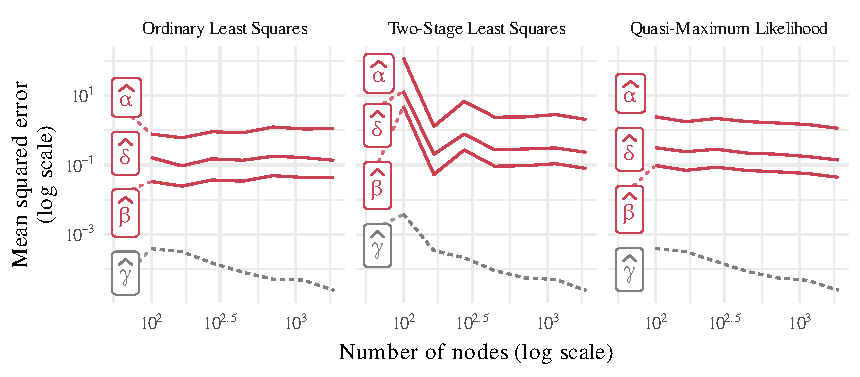
\includegraphics[width=0.8\textwidth]{./figures/simulations/biometrika-mse.pdf}
                    \caption{Mean squared error of estimates. Each panel corresponds to a different estimator. Within a panel, the x-axis represents the sample size on a log scale, and the y-axis represents the Monte Carlo estimate of mean squared error, also on a log scale. Each line corresponds to a single coefficient; solid red lines are asymptotically colinear, dashed gray lines are not.}
                    \label{fig:mse-problem}
                \end{figure}
            \end{block}
        \end{column}

        \separatorcolumn

        \begin{column}{\colwidth}

            \begin{block}{Explanation of the degeneracy}

                \begin{figure}
                    \begin{minipage}{0.49\textwidth}
                        \centering
                        \begin{tikzpicture}
                            \node[shape=circle,fill=MidnightBlue,label=above left:{$T_A = 1$}] (A) at (0,1) {};
                            \node[shape=circle,fill=MidnightBlue,label=below left:{$T_B = 0$}] (B) at (1,0) {};
                            \node[shape=circle,fill=MidnightBlue,label=above right:{$T_C = 1$}] (C) at (1.5,1.5) {};
                            \node[shape=circle,fill=MidnightBlue,label=above right:{$T_D = 1$}] (D) at (2.75,0.5) {};

                            \draw (A) -- (B);
                            \draw (A) -- (C);
                            \draw (B) -- (C);
                            \draw (C) -- (D);
                        \end{tikzpicture}
                    \end{minipage}
                    \begin{minipage}{0.49\textwidth}
                        \centering
                        \begin{tikzpicture}
                            \node[shape=circle,fill=MidnightBlue,label=above left:{$[GT]_A = 1/2$}] (A) at (0,1) {};
                            \node[shape=circle,fill=MidnightBlue,label=below left:{$[GT]_B = 1$}] (B) at (1,0) {};
                            \node[shape=circle,fill=MidnightBlue,label=above right:{$[GT]_C = 2/3$}] (C) at (1.5,1.5) {};
                            \node[shape=circle,fill=MidnightBlue,label=above right:{$[GT]_D = 1$}] (D) at (2.75,0.5) {};

                            \path (A) edge [loop above] node {} (A);
                            \path (B) edge [loop below] node {} (B);
                            \path (C) edge [loop above] node {} (C);
                            \path (D) edge [loop above] node {} (D);

                            \draw (A) -- (B);
                            \draw (A) -- (C);
                            \draw (B) -- (C);
                            \draw (C) -- (D);
                        \end{tikzpicture}
                    \end{minipage}
                    \caption{Neighborhood averaging. (Left) A binary covariate $T$ on small network. (Right) The  average values of $T$ in each node's neighborhood. For example, node $A$ is connected to nodes $B$ and $C$, the average value of $T$ in neighborhood centered on $A$ is $1/2$ (the value of $T$ at node $A$ is excluded from this calculation.). Similarly, the average value of $T$ in the neighborhood centered on $B$ is $1$.}
                    \label{fig:averaging}
                \end{figure}
            \end{block}

            \begin{block}{Semi-parametric network model}


                \begin{lemma} \label{lem:indepcov:nonid}
                    Suppose that (1) the nodal covariates $T_1,T_2,\dots,T_n$ are independent with shared mean $\tau \in \R$, and $T$ is independent of $A$; (2) the centered nodal covariates $\{ T_i - \tau : i \in 1,2,\dots, n \}$, are independent $(\nu,b)$-subgamma random variables; (3) the regression errors $\varepsilon_1, \varepsilon_2, \dots, \varepsilon_n$ are independent subgamma random variables with parameters not depending on $n$, and further are independent of $T_1, ..., T_n$; and (4) the adjacency matrix $A$ contains only non-negative entries and does not contain any self-loops, such that $A_{ii} = 0$ for all $i = 1,2,\dots, n$.

                    If the degrees of the network grow such that
                    \begin{equation} \label{eq:growth:nub}
                        \max_{i \in [n] } \frac{1}{d_i^2} \sum_{j=1}^n A_{ij}^2
                        = o\left( \frac{ 1 }{ \nu \log^2 n } \right)
                        ~\text{ and }
                        \max_{i,j \in [n]} \frac{ A_{ij} }{ d_i }
                        = o\left( \frac{ 1 }{ b \log n } \right).
                    \end{equation}
                    then
                    \begin{equation*}
                        \max_{i \in [n]} \Big\| [GT]_i - \tau \Big\|
                        = o(1) ~ \text{ almost surely }
                    \end{equation*}
                    and
                    \begin{equation*}
                        \max_{i \in [n]} \Big\| [GY]_i - \eta \Big\|
                        = o(1) ~ \text{ almost surely,}
                    \end{equation*}
                    where
                    \begin{equation} \label{eq:def:eta}
                        \eta = \frac{ \alpha + (\gamma+\delta)\tau }{ 1-\beta }.
                    \end{equation}
                \end{lemma}


                \begin{theorem} \label{thm:indepcov:blowup}
                    Let $(\alphahat, \betahat, \gammahat, \deltahat)$ be the vector of ordinary least squares estimates of $(\alpha, \beta, \gamma, \delta)$, based on an $n$-by-$n$ network, and suppose that as $n$ grows, the sequence of networks is such that
                    \begin{equation} \label{eq:frobG:growthbound}
                        \| G \|_F^2 = o( n ).
                    \end{equation}
                    Suppose that the adjacency matrix $A$ contains only non-negative entries and does not contain any self-loops, such that $A_{ii} = 0$ for all $i = 1, 2,\dots, n$; the nodal covariates $T_1,T_2,\dots,T_n$ are independent with shared mean $\tau \in \R$; the regression errors $\varepsilon_1, \varepsilon_2, \dots, \varepsilon_n$ and the centered nodal covariates $\{ T_i - \tau : i =1,2,\dots,n \}$ are independent sub-Gaussian random variables with parameters not depending on $n$; and the vectors $T$ and $\varepsilon$ are independent given $A$.
                    Then if $\beta = 0$,
                    \begin{equation*}
                        \min\{ |\alphahat-\alpha|, |\betahat-\beta| \}
                        = \Omegap{ 1 }
                    \end{equation*}
                    and
                    \begin{equation} \label{eq:deltahat:LB}
                        | \deltahat - \delta | = \Omegap{ \frac{1}{\|G\|_F} }.
                    \end{equation}
                    If $\beta \neq 0$,
                    \begin{equation*}
                        \min\{ |\alphahat-\alpha|, |\betahat-\beta| \}
                        = \Omegap{ \frac{1}{\|G\|_F} }.
                    \end{equation*}
                    Finally, under the stronger growth assumption $\|G\|_F^2 = o( \sqrt{n} )$, equation~\eqref{eq:deltahat:LB} continues to hold for all values of $\beta$.
                \end{theorem}

                TODO
            \end{block}

            \begin{block}{Dependence between network and covariates can fix the degeneracy (partially)}

                \begin{definition}[Random Dot Product Graph]
                    \label{def:rdpg}
                    Let $F$ be a distribution on $\R^d$ such that $0 \le x^T y$ for all $x,y \in \supp F$ and the convex cone of $\supp F$ is $d$-dimensional.
                    Draw $X_1, X_2, \dots, X_n$ independently and identically from $F$, and collect these in the rows of $X \in \R^{n \times d}$ for ease of notation.
                    Conditional on these $n$ vectors, which we call {\em latent positions}, generate edges by drawing $\{ A_{ij} : 1 \le i < j \le n \}$ as independent $(\nu,b)$-subgamma random variables with $\bbE[ A_{ij} \mid X ] = \rho X_i^T X_j$, where $\rho \in [0,1]$.
                    Then we say that $A$ is distributed according to an $n$-vertex random dot product graph with latent position distribution $F$, $(\nu,b)$-subgamma edges and sparsity factor $\rho$.
                    We write $(A,X) \sim \RDPG( F, n)$, with the subgamma and sparsity parameters made clear from the context.
                \end{definition}

                \begin{theorem} \label{thm:rdpg}
                    Suppose that $(A, X)$ are sampled from a random dot product model where $X$ is rank $d$ with probability $1$.
                    Let $\varepsilon$ be a vector of mean zero, i.i.d.~$(\nueps,\beps)$-subgamma random variables, with $(\nueps,\beps)$ not depending on $n$,
                    and let
                    \begin{equation*}
                        Y = \alpha 1_n + \beta G Y + X \gamma + G X \delta + \varepsilon
                    \end{equation*}
                    for $\alpha, \beta \in \R$ and $\gamma, \delta \in \R^d$, and the conditions of Proposition~\ref{prop:bramoulle2009} hold. Suppose that $X$ has $k \ge 2d$ distinct rows. Then, under suitable technical conditions, the columns of design matrix corresponding to $(\alpha, \beta, \delta_1, \delta_2, \dots, \delta_d)$ are asymptotically colinear. If any two elements of $(\alpha, \beta, \delta_1, \delta_2, \dots, \delta_d)$ are equal to zero, there is no asymptotic colinearity.
                \end{theorem}
            \end{block}


        \end{column}

        \separatorcolumn

        \begin{column}{\colwidth}

            \begin{exampleblock}{Theory}
                \begin{figure}
                    \centering
                    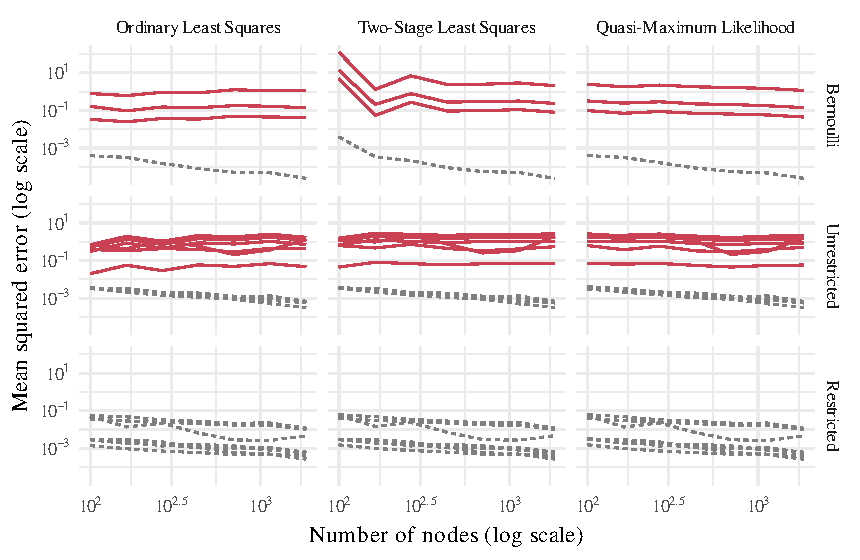
\includegraphics[width=0.8\textwidth]{./figures/simulations/biometrika-mse-all.pdf}
                    \caption{Mean squared error of estimates. Each row of panels denotes a different simulation setting, and each column of panels corresponds to a different estimator. Within a panel, the x-axis represents the sample size on a log scale, and the y-axis represents the Monte Carlo estimate of mean squared error, also on log scale. Each line corresponds to a single coefficient. Solid red lines are asymptotically colinear, dashed gray lines are not.}
                    \label{fig:mse}
                \end{figure}


                \begin{figure}
                    \centering
                    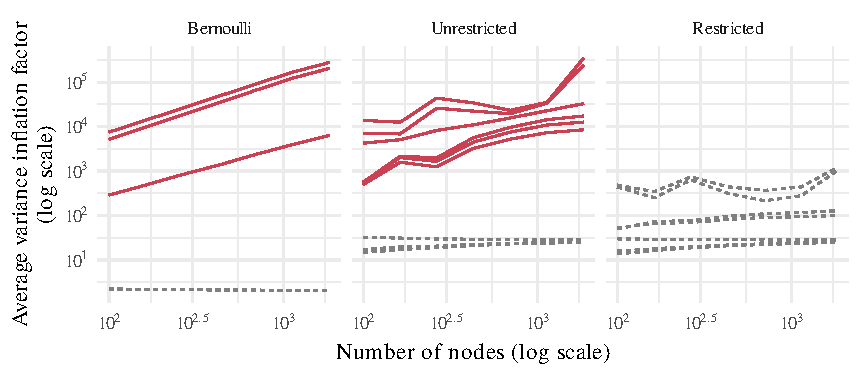
\includegraphics[width=0.8\textwidth]{./figures/simulations/biometrika-vif.pdf}
                    \caption{Average variance inflation factors. Each panel denotes a different simulation setting. The x-axis represents the sample size on a log scale, and the y-axis represents the Monte Carlo estimate of mean variance inflation factor, also on log scale. Each line corresponds to a single coefficient. Solid red lines are asymptotically colinear, dashed gray lines are not.}
                    \label{fig:vif}
                \end{figure}
            \end{exampleblock}

            \begin{alertblock}{Takeaways}
                \begin{enumerate}
                    \item Estimated effects are adjusted for possible confounding by age and church attendance.
                    \item Estimated effects vary with the chosen dimension $d$ of the latent space
                    \item Over-specifying $d$ is typically okay, but under-specifying $d$ leads to a failure to capture social structure in $\X$
                    \item Once we capture enough social structure in $\X$, we see a significant indirect social effect that leads adolescent girls to smoke more
                \end{enumerate}
            \end{alertblock}


            \begin{block}{References \& Contact Info}

                \nocite{hayes2024c}
                \printbibliography

                \begin{center}
                    \url{alex.hayes@wisc.edu} \\
                    \url{https://www.alexpghayes.com}
                \end{center}
            \end{block}


        \end{column}

        \separatorcolumn
    \end{columns}
\end{frame}

\end{document}
